\appendix
\renewcommand\thefigure{A.\arabic{figure}}
\renewcommand\thesection{\Alph{section}}
\renewcommand{\thealgocf}{A.\arabic{algocf}}
\renewcommand\thetable{A.\arabic{table}}
\setcounter{section}{0}
\setcounter{algocf}{0}
%\renewcommand\thealgorithm{A.\arabic{algorithm}}
\setcounter{figure}{0}
\setcounter{table}{0}

\section{Coding Latency}\label{app:coding-latency}

In \cref{tab:latency_per_sequence}, we report the actual encoding and decoding latencies for all sequences in the HiFi4G and N3DV datasets.

\begin{table*}[t]
  \centering
  \footnotesize
  \caption{Encode and decode latency (ms) for video sequences.}
  \label{tab:latency_per_sequence}
  \begin{tabular}{lrrrrrrrrrr}
  \toprule
  Sequence & \multicolumn{2}{c}{\vthree{}-2D} & \multicolumn{2}{c}{MesonGS} & \multicolumn{2}{c}{LTS-Draco} & \multicolumn{2}{c}{G-PCC} & \multicolumn{2}{c}{\gsnfs{} (Ours)} \\
           & Enc & Dec & Enc & Dec & Enc & Dec & Enc & Dec & Enc & Dec \\
  \hline
  Actor1    & 443.1  & 312.5 & 144950.2 & 487.4 & 136.8  & 84.4  & 5063.9  & 2986.5  & 17.4 & 12.8 \\
  Actor2    & 4808.9 & 362.8 & 144363.5 & 368.8 & 103.5  & 60.8  & 3679.6  & 2205.4  & 15.6 & 12.0 \\
  Actor3    & 542.5  & 331.9 & 145057.5 & 529.3 & 156.3  & 95.1  & 6027.0  & 3474.0  & 17.6 & 13.2 \\
  Actor4    & 554.1  & 358.9 & 145351.6 & 622.6 & 182.8  & 104.6 & 8070.4  & 4858.2  & 19.1 & 15.0 \\
  Actor5    & 435.7  & 330.0 & 145003.4 & 559.3 & 158.2  & 91.9  & 5992.8  & 3693.7  & 17.8 & 13.4 \\
  Actor6    & 483.5  & 367.4 & 145344.3 & 674.9 & 201.9  & 113.1 & 8579.4  & 5163.9  & 19.6 & 15.7 \\
  Actor7    & 421.3  & 323.4 & 144602.4 & 504.7 & 151.8  & 88.2  & 5294.2  & 3174.0  & 17.7 & 13.2 \\
  \midrule
  Coffee Martini   & 473.6 & 352.0 & 30228.0 & 1415.6 & 1059.4 & 215.8 & 12540.2 & 10090.6 & 24.9 & 23.9 \\
  Cook Spinach     & 316.8 & 262.8 & 28719.5 & 1012.1 & 229.7  & 127.2 & 7467.1  & 5866.7  & 21.7 & 20.1 \\
  Cut Roasted Beef & 313.3 & 261.0 & 28781.4 & 978.2  & 229.4  & 128.5 & 8162.4  & 6438.3  & 21.5 & 19.6 \\
  Flame Salmon     & 488.0 & 340.3 & 29692.5 & 1335.9 & 413.8  & 214.0 & 11327.0 & 9236.8  & 27.7 & 23.4 \\
  Flame Steak      & 316.9 & 262.3 & 28877.8 & 1080.6 & 222.4  & 129.3 & 6364.7  & 4548.4  & 22.2 & 20.3 \\
  Sear Steak       & 312.8 & 263.2 & 28826.4 & 1061.6 & 247.9  & 133.3 & 6966.3  & 5391.3  & 22.2 & 20.5 \\
  \bottomrule
  \end{tabular}
\end{table*}



\section{\gsnfs{} Octree Encoding}\label{app:sysn-octr-encod}

Algorithm~\ref{algo:octree-encode-gpu} summarizes our GPU octree encoder. Starting from voxelized integer coordinates, we first compute Morton codes for all occupied leaf voxels, then radix-sort and deduplicate them to obtain the leaf set $L_J$. The upper octree levels are constructed bottom-up by repeatedly mapping child codes to their parents and removing duplicates, yielding level-wise node sets $\{L_d\}_{d=0}^J$.

After the hierarchy is built, we serialize a compact occupancy bitstream. The header stores the number of levels and the node count of each level. The payload is then generated in breadth-first order: for each parent in level $L_d$, we produce one occupancy byte indicating which of its eight children are present in $L_{d+1}$. As shown in Algorithm~\ref{algo:octree-encode-gpu}, this is done by locating the base child Morton code and setting the corresponding bits for all valid children in the next level.

This construction avoids explicit pointer-based octree data structures and operates directly on sorted Morton codes, which is well suited to parallel primitives such as radix sort, deduplication, and batched searches. The resulting bitstream is a level-synchronous octree representation that can be decoded with the same breadth-first traversal order.

\begin{algorithm}[t]
  \caption{GPU Octree{}'s Encoding from Voxelized Positions}
  \label{algo:octree-encode-gpu}
\SetAlgoLined
\DontPrintSemicolon

\SetKwInOut{Input}{Input}
\SetKwInOut{Output}{Output}

\SetKwFunction{Morton}{Morton}
\SetKwFunction{RadixSort}{RadixSort}
\SetKwFunction{Unique}{Unique}
\SetKwFunction{Parent}{Parent}
\SetKwFunction{OccKernel}{OccKernel}
\SetKwFunction{Concat}{Concat}
\SetKwFunction{Append}{Append}
\SetKwFunction{BinarySearch}{BinarySearch}

\Input{Voxelized integer positions $\hat{V}=\{(\hat{x}_i,\hat{y}_i,\hat{z}_i)\}_{i=1}^{\hat{N}_v}$ on GPU; octree depth $J$}
\Output{Serialized octree bitstream $B_{occ}$}

\BlankLine
\tcp*[l]{Step 1: Morton codes for leaf voxels}
\ForPar{$i \gets 1$ \KwTo $\hat{N}_v$}{
  $m_i \gets \Morton(\hat{x}_i,\hat{y}_i,\hat{z}_i, J)$
}
$L_J \gets \Unique(\RadixSort(\{m_i\}))$ \tcp*{leaf nodes}

\BlankLine
\tcp*[l]{Step 2: Level-synchronous octree construction}
\For(\tcp*[f]{bottom-up parents}){$d \gets J-1$ \KwTo $0$}{
  $L_d \gets \Unique(\{\, \Parent(c_m)\;|\;c_m\in L_{d+1}\,\})$ \tcp*{$\Parent(c_m)=c_m\gg 3$}
}

\BlankLine
\tcp*[l]{Step 3: Bitstream header}
$num\_levels \gets J+1$\;
$level\_sizes \gets (|L_0|,\ldots,|L_J|)$\;
$B_{occ} \gets \Append(B_{occ}, num\_levels, level\_sizes)$\;

\BlankLine
\tcp*[l]{Step 4: Breadth-first occupancy bitstream.}
\ForPar{$d \gets 0$ \KwTo $J-1$}{
  $B_d \gets \OccKernel(L_d, L_{d+1})$
  $B_{occ} \gets \Append(B_{occ}, B_d)$ \tcp*{contiguous bytes for level $d$}
}

\Return $B_{occ}$\;

\BlankLine
\textbf{Kernel \OccKernel($L_d,L_{d+1}$):}\;
\ForPar{$p \in L_d$}{
  $c_m^b \gets p \ll 3$ \tcp*{base child code}
  $occ \gets 0$ \tcp*{occupancy byte}
  $c_m \gets \BinarySearch(L_{d+1}, c_m^b)$
  \For{$k \gets 0$ \KwTo $7$}{
      \If{$L_{d+1}[c_m+k] \leq c_m^b+7$}{
        $occ \gets occ \;|\; \big(1 \ll (L_{d+1}[c_m+k]-c_m^b)\big)$\;
      }
      
  }
  Write $occ$ into $B_d$ at parent's index\;
}
\end{algorithm}


\section{\gsnfs{}'s Octree Decoding}\label{app:sysn-octr-decod}
\begin{algorithm}[t]
  \caption{GPU Octree Decoding}
  \label{algo:octree-decode-gpu}
\SetAlgoLined
\DontPrintSemicolon

\SetKwInOut{Input}{Input}
\SetKwInOut{Output}{Output}

\SetKwFunction{ReadHeader}{ReadHeader}
\SetKwFunction{ReadOcc}{ReadOccBytes}
\SetKwFunction{Popcount}{Popcount}
\SetKwFunction{ExScan}{ExclusiveScan}
\SetKwFunction{ExpandKernel}{ExpandChildrenKernel}
\SetKwFunction{ReconKernel}{ReconstructPointsKernel}
\SetKwFunction{MortonDec}{MortonDecode}
\SetKwFunction{Interleave}{InterleaveXYZ}

\Input{Compressed octree buffer $B$ on GPU; octree depth $J$}
\Output{Voxelized positions $\hat{V}$ on GPU; leaf Morton codes $L_J$ on GPU}
\BlankLine
\tcp*[l]{Step 1: Parse header.}
$(num\_levels,\ level\_sizes,\ ptr) \gets \ReadHeader(B)$\;

\BlankLine
\tcp*[l]{Step 2: Initialize root list (implicit root Morton code).}
$L_0 \gets [\,0\,]$

\BlankLine
\tcp*[l]{Step 3: Level-synchronous decoding.}
\For(\tcp*[f]{top-down levels}){$d \gets 0$ \KwTo $J-1$}{
  $M_d \gets |L_d|$\;
  $Occ_d \gets \ReadOcc(ptr, M_d)$ \tcp*{read $M_d$ bytes from $B$ into a GPU array}
  $ptr \gets ptr + M_d$\;

  \BlankLine
  \tcp*[l]{Count children per parent.}
  \ForPar{$p \gets 1$ \KwTo $M_d$}{
    $cnt[p] \gets \Popcount(Occ_d[p])$\;
  }

  \BlankLine
  \tcp*[l]{Find total children at $d+1$.}
  $off \gets \ExScan(cnt)$
  $T \gets off[M_d] + cnt[M_d]$\;
  Allocate $L_{d+1}$ of length $T$\;

  \BlankLine
  \tcp*[l]{Expand children.}
  \ExpandKernel$(L_d, Occ_d, off, L_{d+1})$ with $M_d$ threads\;
}

\BlankLine
\tcp*[l]{Step 6: Get voxel coordinates at leaf.}
$\hat{N}_v \gets |L_J|$\;
$shift \gets J_v - J$\;
Allocate $\hat{x}[1{:}\hat{N}_v],\hat{y}[1{:}\hat{N}_v],\hat{z}[1{:}\hat{N}_v]$\;
Launch \ReconKernel$(L_J, shift, \hat{x},\hat{y},\hat{z})$ with $\hat{N}_v$ threads\;
$\hat{V} \gets \Interleave(\hat{x},\hat{y},\hat{z})$ \tcp*{Reverse Morton Code.}

\Return $(\hat{V}, L_J)$\;
\end{algorithm}

\begin{algorithm}[h!]
  \caption{\texttt{expand\_children\_kernel}: Expand occupied children and generate Morton codes}
  \label{algo:octree-expand-children-kernel}
\SetAlgoLined
\DontPrintSemicolon
\SetKwInOut{Input}{Input}
\SetKwInOut{Output}{Output}

\Input{Parent Morton codes $L_d[1{:}M_d]$; occupancy bytes $Occ_d[1{:}M_d]$; write offsets $off[1{:}M_d]$}
\Output{Child Morton codes $L_{d+1}[1{:}T]$}

\ForPar{$p \gets 1$ \KwTo $M_d$}{
  $parent \gets L_d[p]$\;
  $occ \gets Occ_d[p]$\;
  $base \gets parent \ll 3$ \tcp*{base child Morton code}
  $w \gets off[p]$ \tcp*{exclusive-scan start offset for this parent}
  \For{$i \gets 0$ \KwTo $7$}{
    \If{$occ \wedge (1 \ll i)$}{
      $L_{d+1}[w] \gets base + i$\;
      $w \gets w + 1$\;
    }
  }
}
\end{algorithm}
The GPU decoder reconstructs voxelized geometry by replaying the serialized occupancy stream in a level-synchronous manner, without building any explicit tree pointers.
%
Starting from the implicit root Morton code ($L_0=\{0\}$), for each depth $d$ it reads the $|L_d|$ occupancy bytes, counts the number of occupied children per parent (population count), and performs an exclusive prefix-sum to compute disjoint write offsets for the next-level array.
%
It then launches \texttt{expand\_children\_kernel} (Alg.~\ref{algo:octree-expand-children-kernel}), which generates each occupied child Morton code in $O(1)$ via $(parent \ll 3)+i$ and writes all children contiguously into $L_{d+1}$, avoiding atomics despite variable fan-out.
%
Repeating this from $d=0$ to $J{-}1$ yields the leaf Morton codes $L_J$, which are finally decoded into integer voxel coordinates (and optionally interleaved) in a parallel post-pass.
%
Overall, decoding preserves the same breadth-first structure as the encoder while turning the key sequential dependency (unknown next-level size) into a standard GPU pattern: count $\rightarrow$ prefix-sum $\rightarrow$ parallel scatter.
%
Full algorithm can be found here~\ref{algo:octree-decode-gpu}.

\section{\gsnfs{}'s RAHT Implementation}\label{app:sysn-raht-encod}

We implement RAHT as a two-stage GPU pipeline: a \emph{prelude} that builds the merge schedule from Morton-sorted occupied voxels, and a \emph{transform} stage that applies the weighted orthonormal rotations using that schedule. This separation isolates the octree-dependent control flow from the per-attribute transform, allowing the latter to be executed with simple parallel kernels.

Algorithm~\ref{algo:raht-prelude} gives the reference non-parallel prelude. For each of the $3J$ binary merge steps induced by a depth-$J$ octree, it constructs the active index list $I_\ell$, the corresponding run-length weights $W_\ell$, and the sibling flags $F_\ell$. Here, $W_\ell$ records the number of original voxels represented by each active entry, and $F_\ell$ marks whether an entry is the left element of a valid sibling pair. The sibling relation is tested directly from Morton codes using XOR and a level-dependent mask, without explicitly materializing the octree.

Algorithm~\ref{algo:raht-prelude-gpu} shows the GPU version of this schedule construction. At each level, one thread computes the weight and sibling flag for one active entry. The next active list is then obtained by removing right siblings while keeping left siblings and singletons. This produces the schedule $[(I_\ell, W_\ell, F_\ell)]_{\ell=1}^{3J}$ used by the transform.

Algorithm~\ref{algo:raht-forward} applies the forward or inverse RAHT on the GPU. In the forward pass, levels are processed bottom-up; in the inverse pass, they are processed in reverse order. For each sibling pair, the transform uses the standard RAHT weights
$$
a=\sqrt{\frac{w_0}{w_0+w_1}}, \qquad
b=\sqrt{\frac{w_1}{w_0+w_1}},
$$
to perform the corresponding orthonormal rotation independently for each attribute channel. Since pairs within a level are disjoint, the computation can be parallelized across active entries.


\begin{algorithm}[h!]
  \caption{RAHT prelude (non-parallel)}
  \label{algo:raht-prelude}
\SetAlgoLined
\DontPrintSemicolon
\SetKwInOut{Input}{Input}
\SetKwInOut{Output}{Output}

\Input{Morton codes $M[0{:}N_v{-}1]$, Num voxels $N_v$, octree depth $J$}
\Output{$[(I_\ell, W_\ell, F_\ell)]_{\ell=1}^{3J}$}

\For{$\ell \gets 1$ \KwTo $3J$}{
  \uIf{$\ell = 1$}{
    $I_1 \gets (0{:}N_v{-}1)^{T}$ \tcp*{active indices at level 1}
  }\Else{
    $I_\ell \gets I_{\ell-1}\big(\neg [0; F_{\ell-1}]\big)$ \tcp*{keep left siblings + singletons}
  }
  $M_\ell \gets M[I_\ell]$ \tcp*{Morton codes at level $\ell$}
  $W_\ell \gets [I_\ell(2{:}\mathrm{end});\, N_v] - I_\ell$ \tcp*{run-length weights (sentinel $N_v$)}
  $D \gets M_\ell(1{:}\mathrm{end}{-}1)\ \oplus\ M_\ell(2{:}\mathrm{end})$ \tcp*{path diffs}
  $F_\ell \gets \big(D\ \wedge\ (2^{3J} - 2^{\ell})\big) = 0$ \tcp*{left-sibling flags}
}
\Return $[(I_\ell, W_\ell, F_\ell)]_{\ell=1}^{3J}$\;
\end{algorithm}

\begin{algorithm}[t]
  \caption{RAHT Prelude on GPU}
  \label{algo:raht-prelude-gpu}
\SetAlgoLined
\DontPrintSemicolon
\SetKwInOut{Input}{Input}
\SetKwInOut{Output}{Output}
\SetKwFunction{Shift}{torch.shift}
\SetKwFunction{MaskedSelect}{torch.masked\_select}
\SetKwFunction{FWKernel}{FWKernel}

\Input{Morton codes $M[0{:}N_v{-}1]$, Num voxels $N_v$, octree depth $J$}
\Output{$[(I_\ell, W_\ell, F_\ell)]_{\ell=1}^{3J}$}

$I_1 \gets (0{:}N_v{-}1)^{T}$\;
\For{$\ell \gets 1$ \KwTo $3J$}{
  $\mu_\ell \gets (2^{3J} - 2^{\ell})$ \tcp*{mask for sibling test}
  % $end \gets N_v$ \tcp*{sentinel for run-length weights}
  \ForPar(\tcp*[f]{1 GPU thread per $k$}){$k \gets 1$ \KwTo $M_\ell$}{
    $curr \gets I_\ell(k)$\;
    $next \gets \begin{cases}
      end & \text{if } k = M_\ell\\
      I_\ell(k{+}1) & \text{otherwise}
    \end{cases}$\;

    $W_\ell(k) \gets next - curr$\;

    \uIf{$k = M_\ell$}{
      $F_\ell(k) \gets 0$\;
    }\Else{
      $F_\ell(k) \gets ((M(curr) \oplus M(next)) \wedge \mu_\ell ) = 0$\;
    }
  }

  $P_\ell \gets \Shift(F_\ell)$ \tcp*{$[0; F_\ell(0{:}\mathrm{end}{-}1)]$ marks right siblings}
  $I_{\ell+1} \gets \MaskedSelect(I_\ell, \neg P_\ell)$

  \If{$|I_{\ell+1}| = 1$}{
    % $L \gets \ell$\;
    \textbf{break}\;
  }
}
\Return $[(I_\ell, W_\ell, F_\ell)]_{\ell=1}^{3J}$\;
\end{algorithm}

% \begin{algorithm}[t]
%   \caption{\textsc{FWKernel}: Compute $(W_\ell,F_\ell)$ on GPU}
%   \label{algo:raht-fwkernel}
% \SetAlgoLined
% \DontPrintSemicolon
% \SetKwInOut{Input}{Input}
% \SetKwInOut{Output}{Output}

% \Input{Index list $I_\ell$ (len $M_\ell$), Morton codes $M$, mask $\mu_\ell$, end sentinel $end$}
% \Output{Weights $W_\ell$ (len $M_\ell$), Flags $F_\ell$ (len $M_\ell$)}

% \ForPar(\tcp*[f]{1 GPU thread per $k$}){$k \gets 1$ \KwTo $M_\ell$}{
%   $curr \gets I_\ell(k)$\;
%   $next \gets \begin{cases}
%     end & \text{if } k = M_\ell\\
%     I_\ell(k{+}1) & \text{otherwise}
%   \end{cases}$\;

%   $W_\ell(k) \gets next - curr$\;

%   \uIf{$k = M_\ell$}{
%     $F_\ell(k) \gets 0$\;
%   }\Else{
%     $F_\ell(k) \gets ((M(curr) \oplus M(next)) \wedge \mu_\ell ) = 0$\;
%   }
% }
% \Return $(W_\ell,F_\ell)$\;
% \end{algorithm}

\begin{algorithm}[h!]
\caption{RAHT Transform (Forward / Inverse) on GPU}
\label{algo:raht-forward}
\SetAlgoLined
\DontPrintSemicolon
\SetKwInOut{Input}{Input}
\SetKwInOut{Output}{Output}

\Input{Attributes $A\in\mathbb{R}^{N_v\times C}$ (GPU), prelude schedule $[(I_\ell,W_\ell,F_\ell)]_{\ell=1}^{3J}$, \texttt{inverse} flag}
\Output{Coefficients $Y\in\mathbb{R}^{N_v\times C}$ (GPU)}

$Y \gets A$ \tcp*{clone for in-place updates}
\If{\texttt{inverse} = 0}{
  \For(\tcp*[f]{bottom-up}){$\ell \gets 1$ \KwTo $3J-1$}{
    $M_\ell \gets |I_\ell|$\;
    Launch \texttt{raht\_forward\_level\_kernel} with $M_\ell$ threads\;
    \Indp
    \ForPar{$k \gets 0$ \KwTo $M_\ell-2$}{
      \If{$F_\ell[k]$}{
        $i_0 \gets I_\ell[k]$;\;
        $i_1 \gets I_\ell[k+1]$;\;
        $w_0 \gets W_\ell[k]$;\;
        $w_1 \gets W_\ell[k+1]$;\;
        $a \gets \sqrt{w_0/(w_0+w_1)}$;\;
        $b \gets \sqrt{w_1/(w_0+w_1)}$;\;
        \For{$c \gets 0$ \KwTo $C-1$}{
          $y_0 \gets Y[i_0,c]$;\;
          $y_1 \gets Y[i_1,c]$;\;
          $Y[i_0,c] \gets a\cdot y_0 + b\cdot y_1$\;
          $Y[i_1,c] \gets -b\cdot y_0 + a\cdot y_1$\;
        }
      }
    }
    \Indm
  }
}{
  \For(\tcp*[f]{top-down}){$\ell \gets 3J-1$ \KwTo $1$}{
    $M_\ell \gets |I_\ell|$\;
    Launch \texttt{raht\_inverse\_level\_kernel} with $M_\ell$ threads\;
    \Indp
    \ForPar{$k \gets 0$ \KwTo $M_\ell-2$}{
      \If{$F_\ell[k]$}{
        $i_0 \gets I_\ell[k]$;\;
        $i_1 \gets I_\ell[k+1]$;\;
        $w_0 \gets W_\ell[k]$;\;
        $w_1 \gets W_\ell[k+1]$;\;
        $a \gets \sqrt{w_0/(w_0+w_1)}$;\;
        $b \gets \sqrt{w_1/(w_0+w_1)}$;\;
        \For{$c \gets 0$ \KwTo $C-1$}{
          $y_0 \gets Y[i_0,c]$;\;
          $y_1 \gets Y[i_1,c]$;\;
          $Y[i_0,c] \gets a\cdot y_0 - b\cdot y_1$\;
          $Y[i_1,c] \gets b\cdot y_0 + a\cdot y_1$\;
        }
      }
    }
    \Indm
  }
}
\Return $Y$\;
\end{algorithm}


\section{R-D Curves}

This section provides the per-sequence R-D curves for all evaluated methods. For completeness, we include one representative frame from each sequence and plot the corresponding bitrate--quality trade-off. Figures~\ref{fig:rd-baselines-hifi4g} and~\ref{fig:rd-baselines-n3dv} report the results for the HiFi4G and N3DV datasets, respectively.

\begin{figure}[htbp]
    \centering
    \begin{subfigure}[b]{0.48\linewidth}
        \centering
        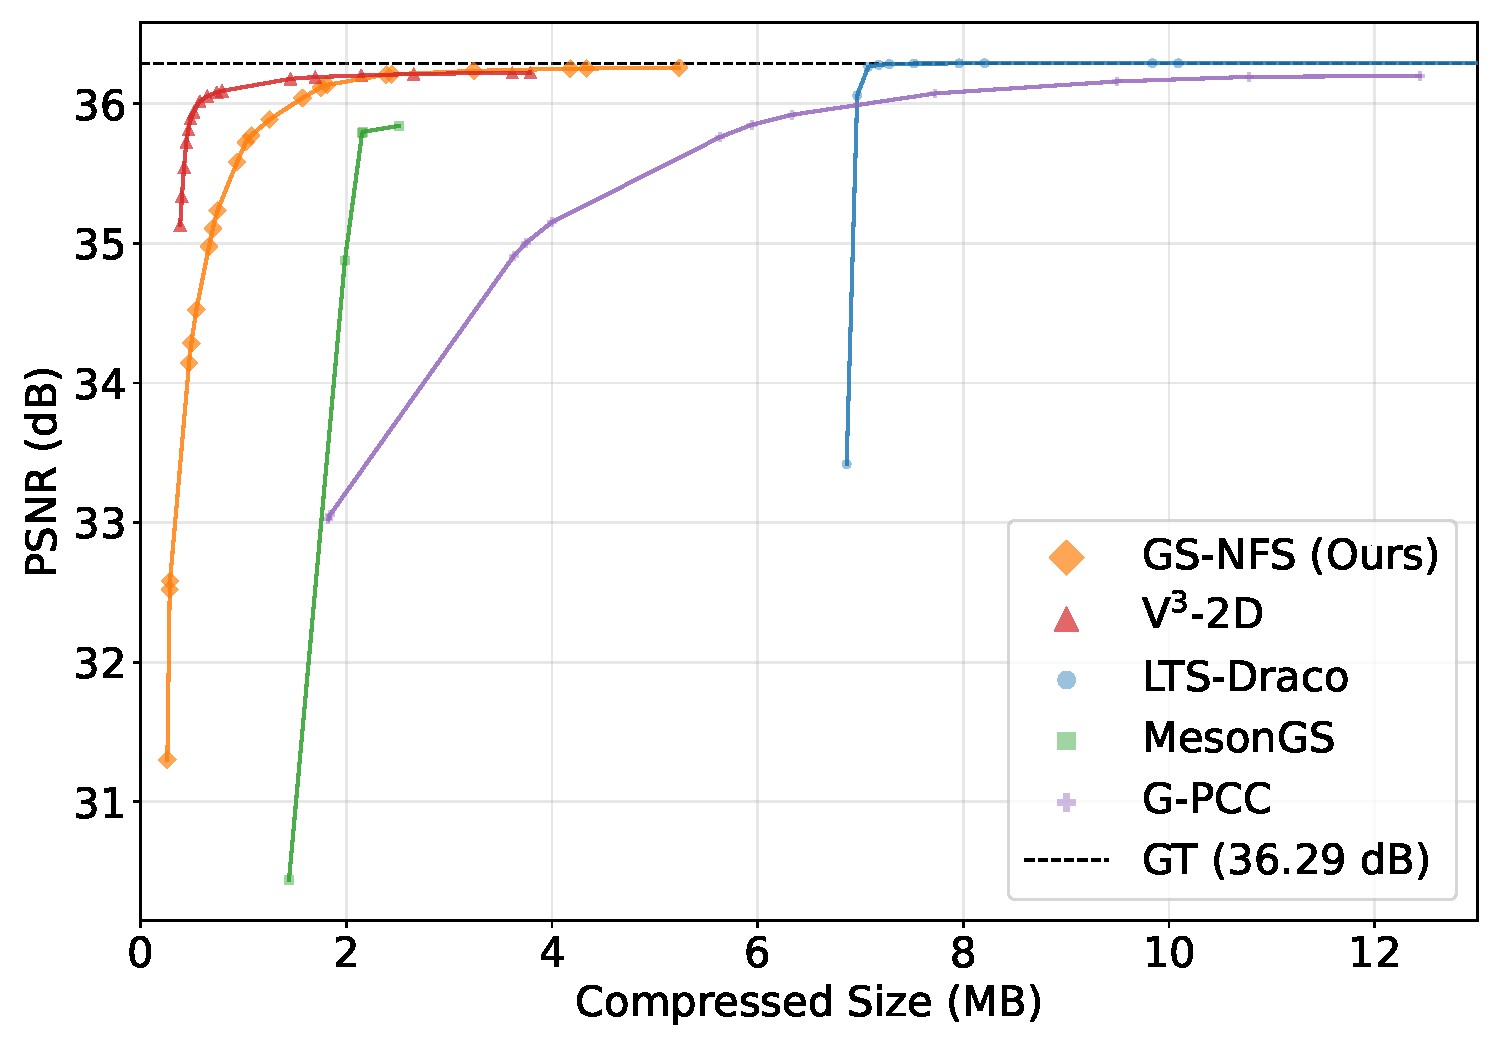
\includegraphics[width=\linewidth]{figures/rd_baselines/rd_baselines_curve_4K_Actor1_Greeting_frame0.pdf}
        \caption{Actor1\_Greeting}
        \label{fig:rd-actor1-greeting}
    \end{subfigure}
    \hfill
    \begin{subfigure}[b]{0.48\linewidth}
        \centering
        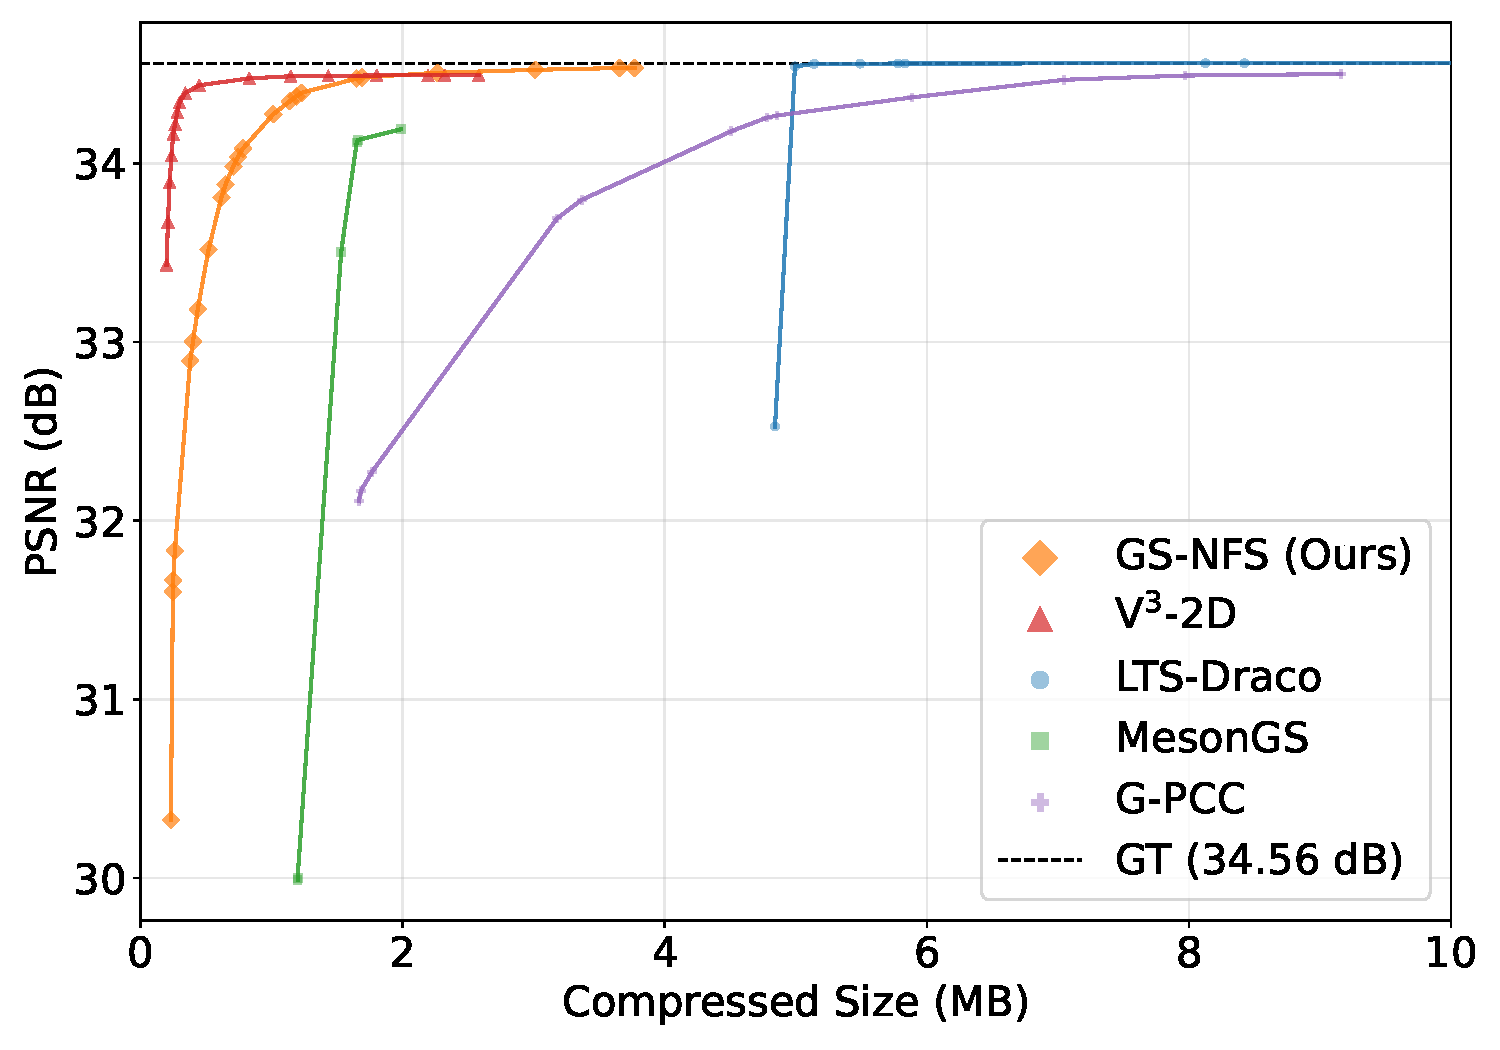
\includegraphics[width=\linewidth]{figures/rd_baselines/rd_baselines_curve_4K_Actor2_Dancing_frame0.pdf}
        \caption{Actor2\_Dancing}
        \label{fig:rd-actor2-dancing}
    \end{subfigure}
    \vspace{0.5em}
    \begin{subfigure}[b]{0.48\linewidth}
        \centering
        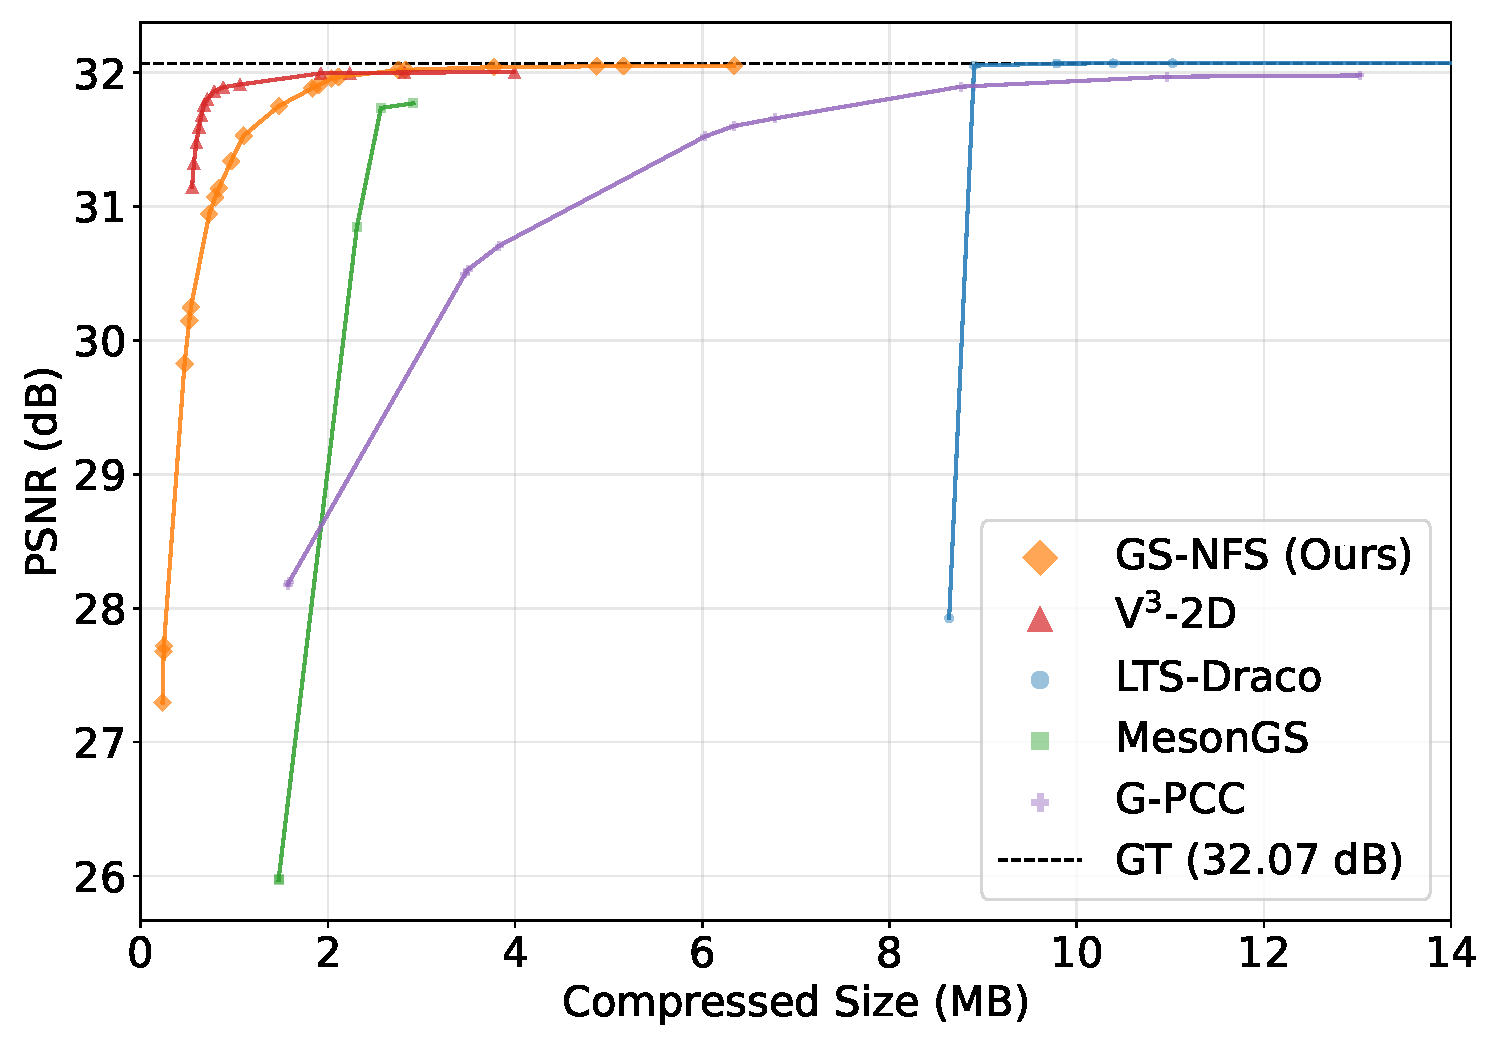
\includegraphics[width=\linewidth]{figures/rd_baselines/rd_baselines_curve_4K_Actor3_Violin_frame0.pdf}
        \caption{Actor3\_Violin}
        \label{fig:rd-actor3-violin}
    \end{subfigure}
    \hfill
    \begin{subfigure}[b]{0.48\linewidth}
        \centering
        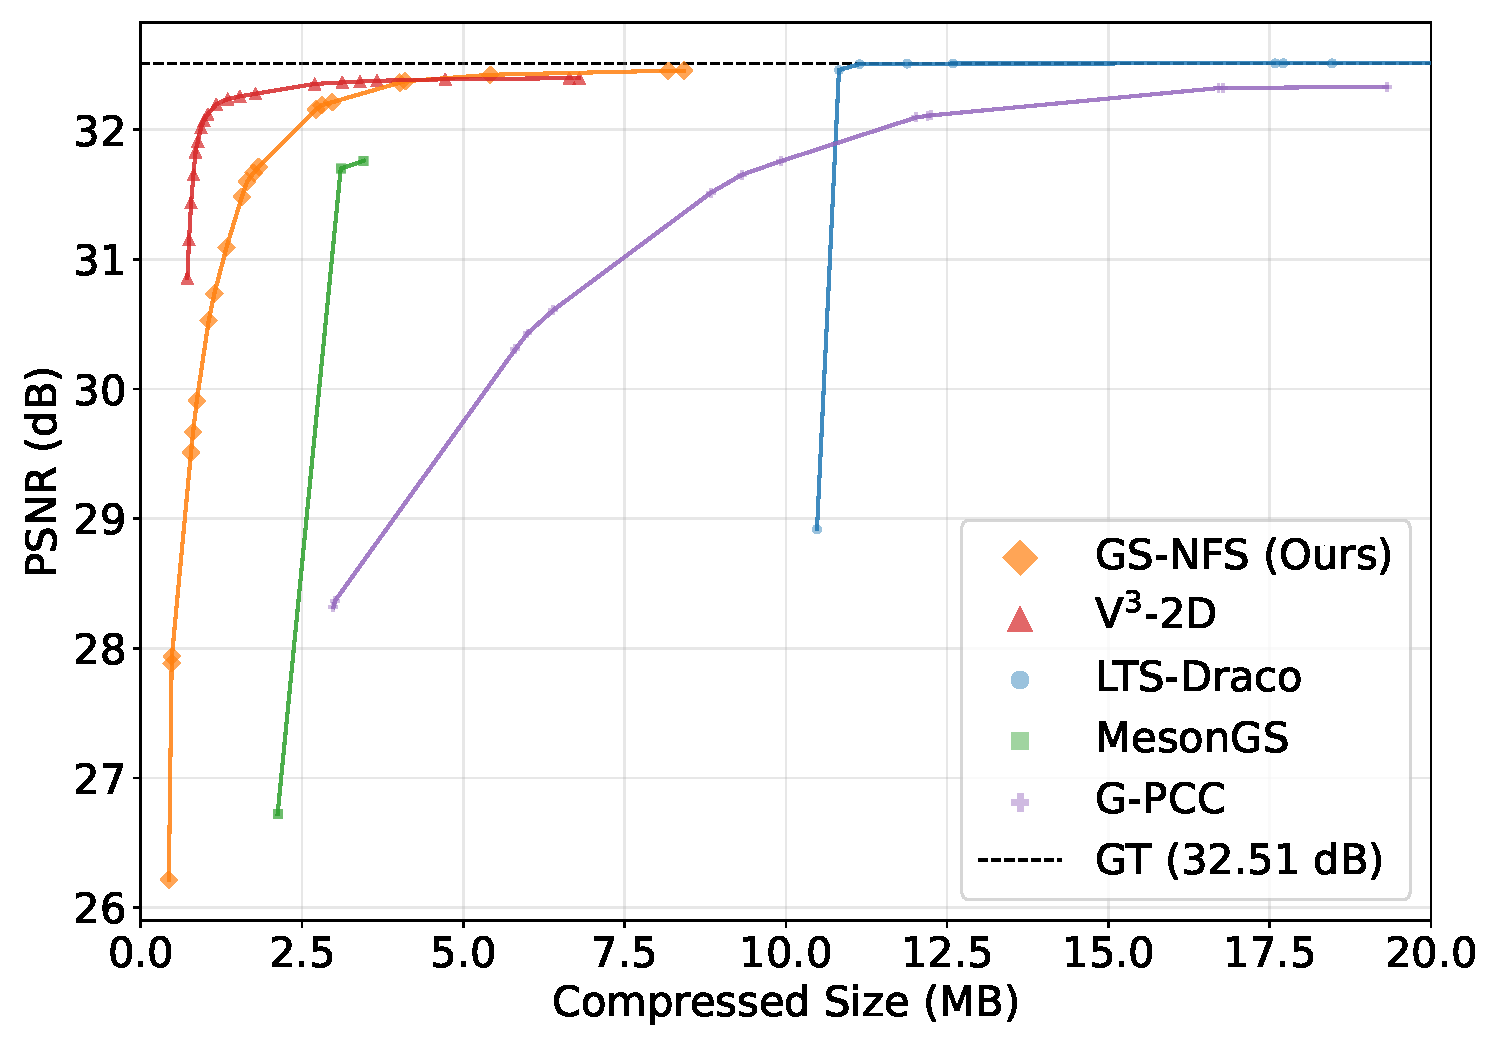
\includegraphics[width=\linewidth]{figures/rd_baselines/rd_baselines_curve_4K_Actor4_Dancing_frame0.pdf}
        \caption{Actor4\_Dancing}
        \label{fig:rd-actor4-dancing}
    \end{subfigure}
    \vspace{0.5em}
    \begin{subfigure}[b]{0.48\linewidth}
        \centering
        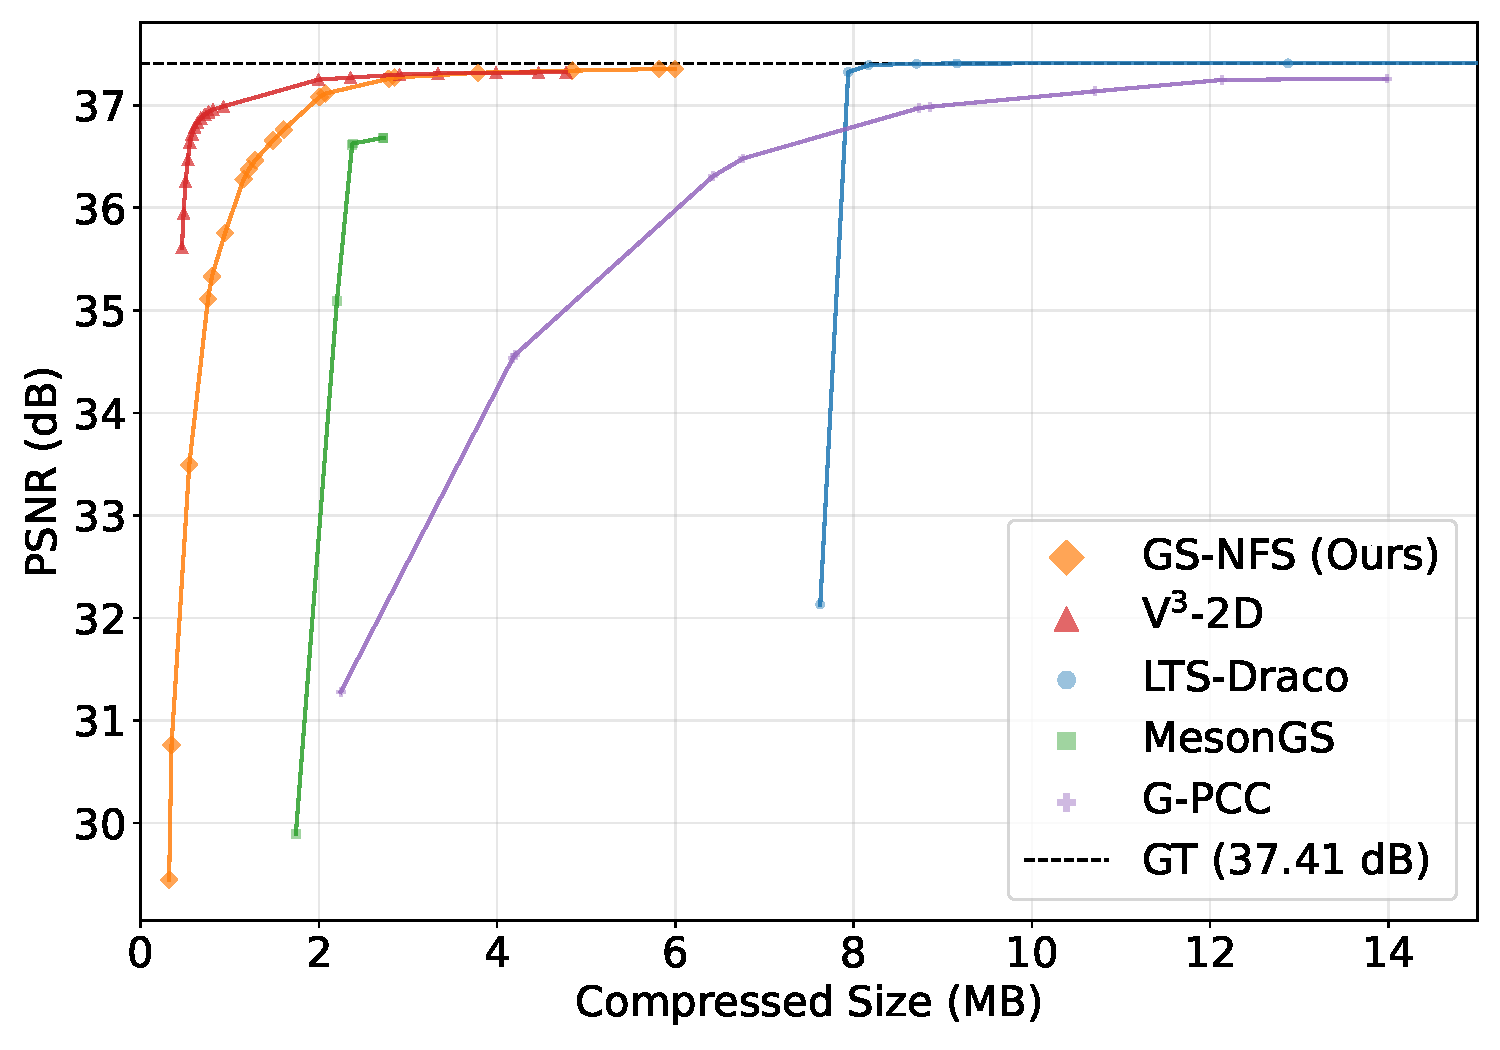
\includegraphics[width=\linewidth]{figures/rd_baselines/rd_baselines_curve_4K_Actor5_Oil-paper_Umbrella_frame0.pdf}
        \caption{Actor5\_Oil-paper\_Umbrella}
        \label{fig:rd-actor5-umbrella}
    \end{subfigure}
    \hfill
    \begin{subfigure}[b]{0.48\linewidth}
        \centering
        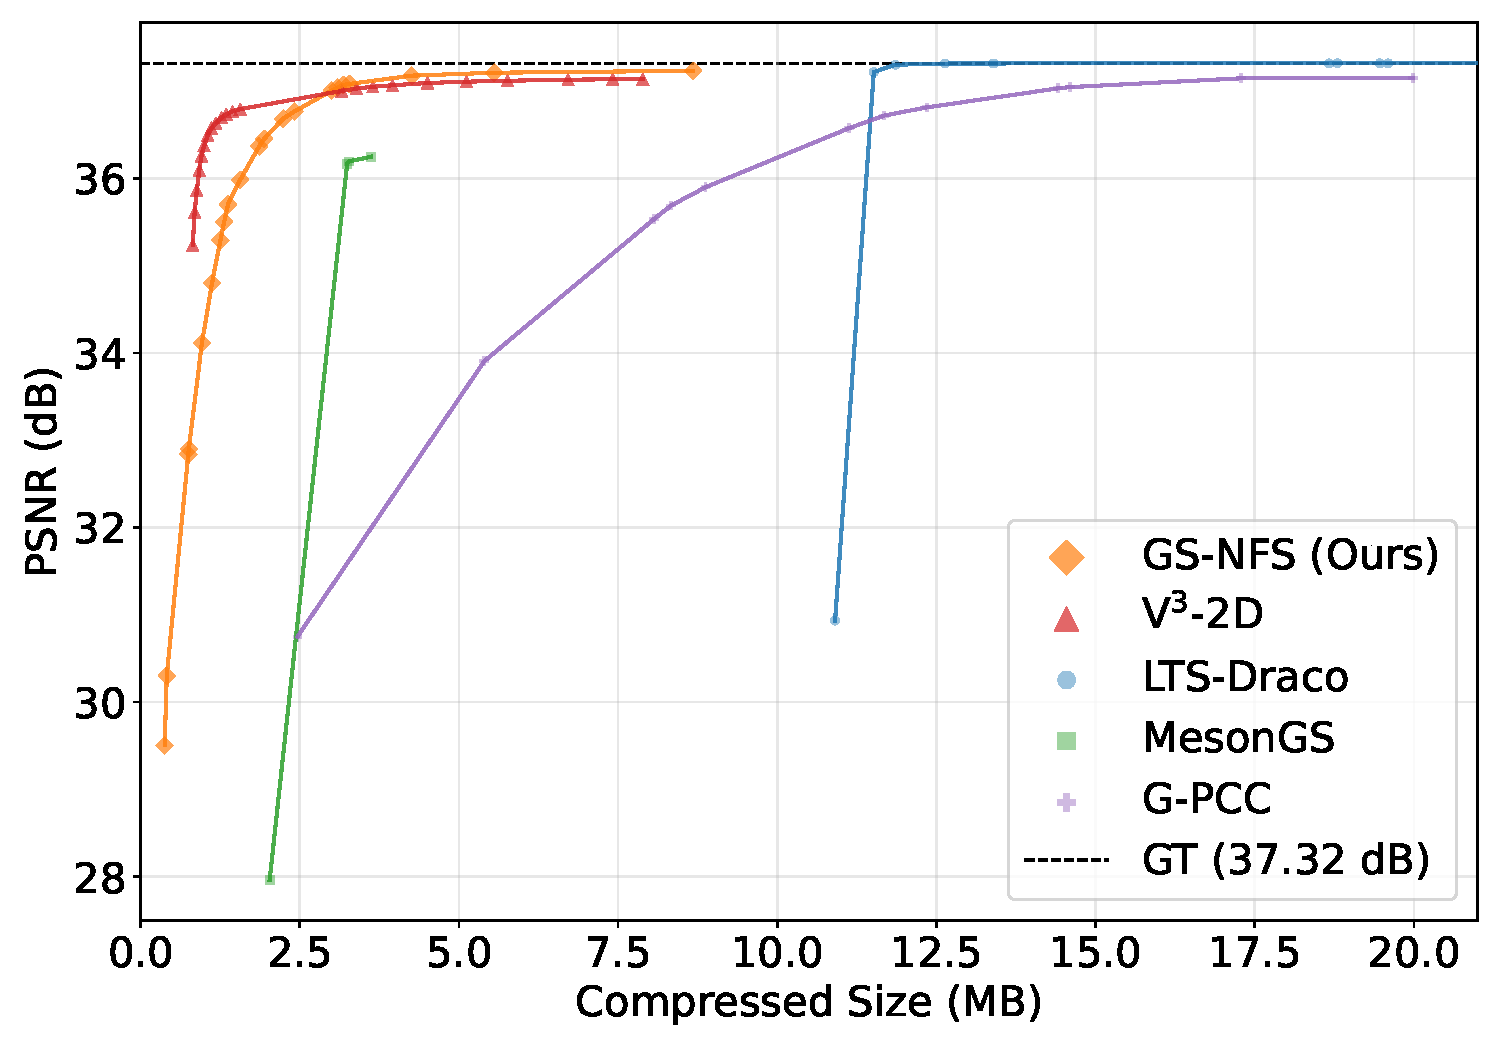
\includegraphics[width=\linewidth]{figures/rd_baselines/rd_baselines_curve_4K_Actor6_Changing_Clothes_frame0.pdf}
        \caption{Actor6\_Changing\_Clothes}
        \label{fig:rd-actor6-clothes}
    \end{subfigure}
    \vspace{0.5em}
    \begin{subfigure}[b]{0.48\linewidth}
        \centering
        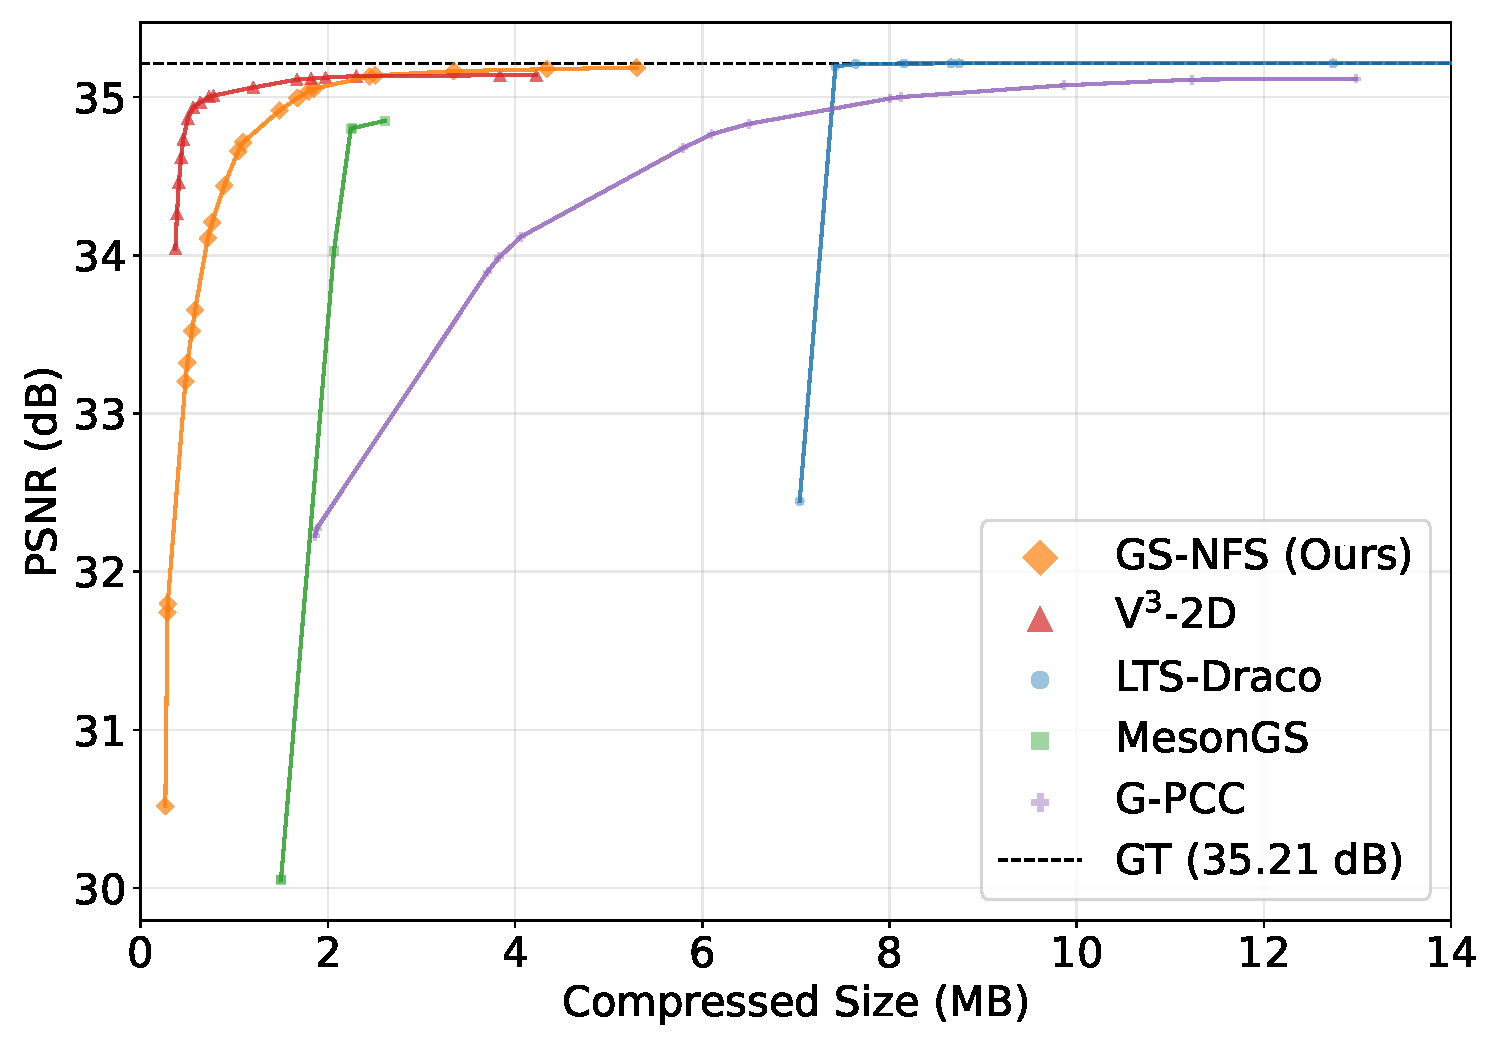
\includegraphics[width=\linewidth]{figures/rd_baselines/rd_baselines_curve_4K_Actor7_Nunchaku_frame0.pdf}
        \caption{Actor7\_Nunchaku}
        \label{fig:rd-actor7-nunchaku}
    \end{subfigure}
    \caption{Rate-distortion curves for HiFi4G 4K sequences (frame 0).}
    \label{fig:rd-baselines-hifi4g}
\end{figure}
\begin{figure}[htbp]
    \centering
    \begin{subfigure}[b]{0.48\linewidth}
        \centering
        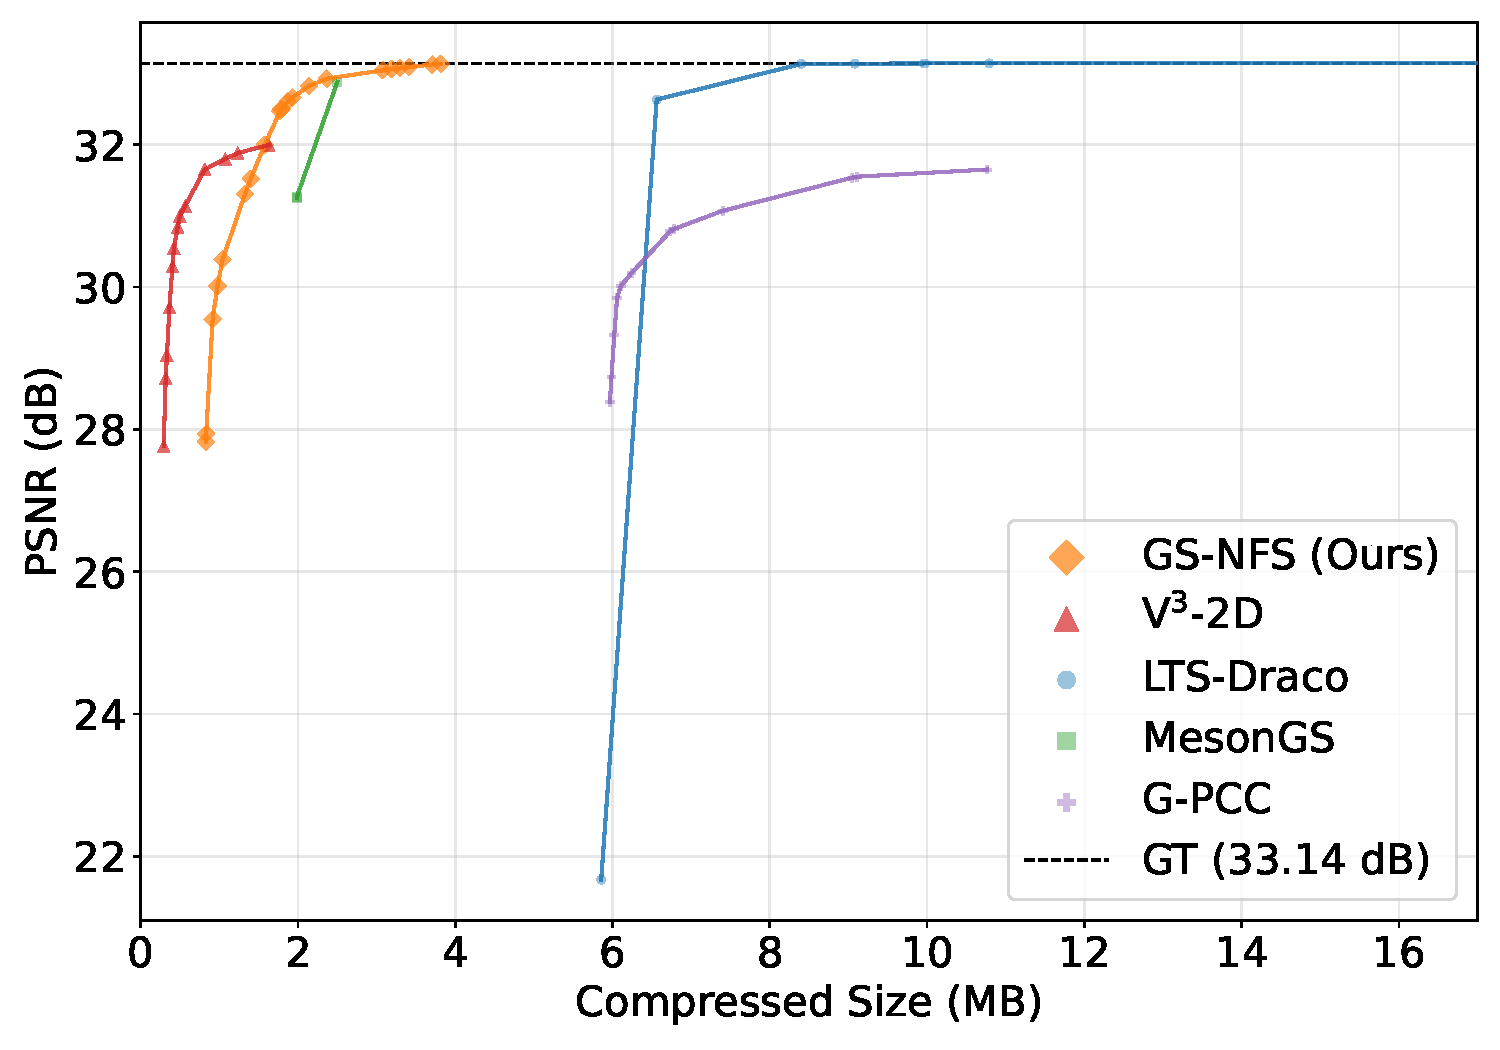
\includegraphics[width=\linewidth]{figures/rd_baselines/rd_baselines_curve_cook_spinach_frame1.pdf}
        \caption{cook\_spinach}
        \label{fig:rd-cook-spinach}
    \end{subfigure}
    \hfill
    \begin{subfigure}[b]{0.48\linewidth}
        \centering
        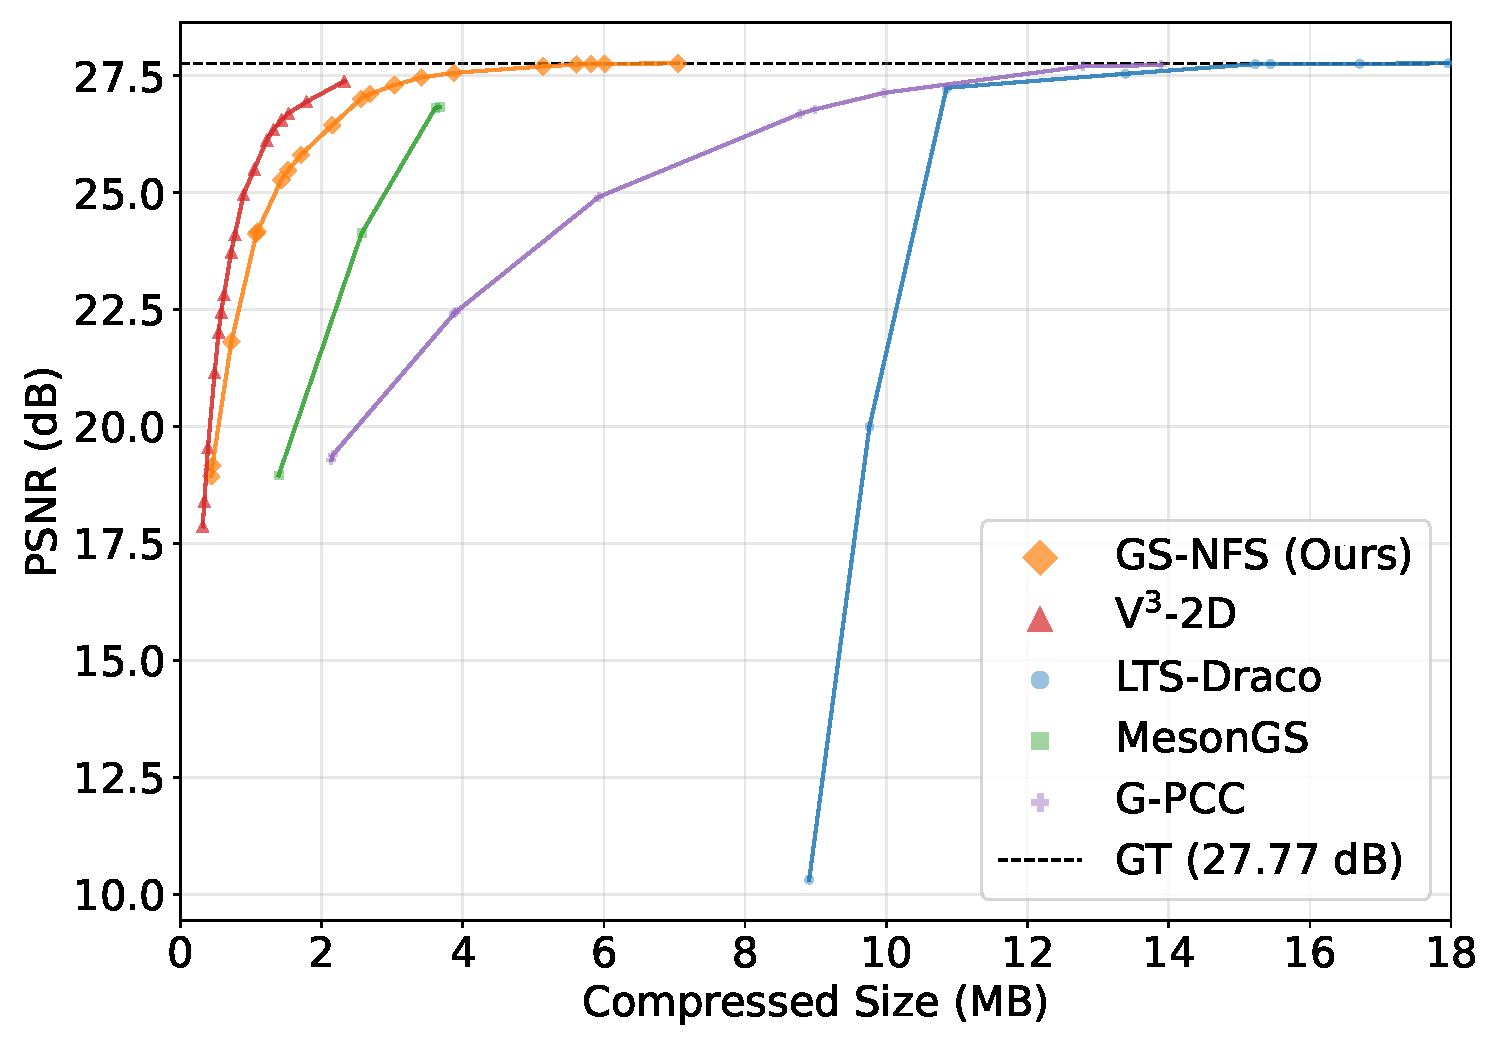
\includegraphics[width=\linewidth]{figures/rd_baselines/rd_baselines_curve_coffee_martini_frame1.pdf}
        \caption{coffee\_martini}
        \label{fig:rd-coffee-martini}
    \end{subfigure}
    \vspace{0.5em}
    \begin{subfigure}[b]{0.48\linewidth}
        \centering
        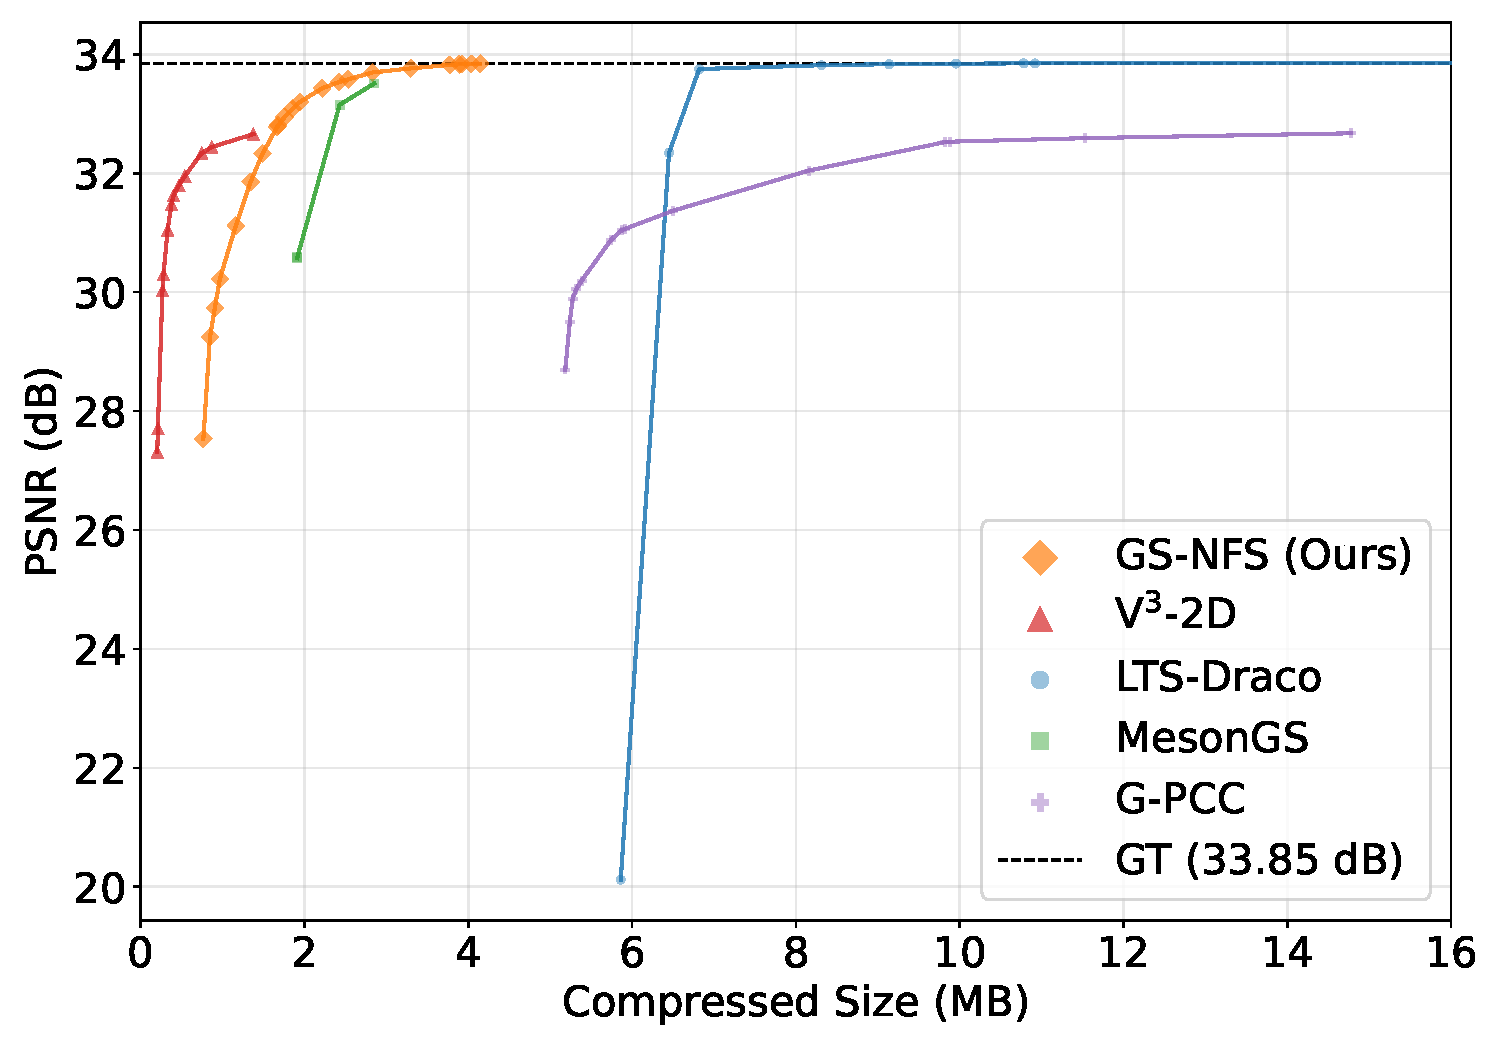
\includegraphics[width=\linewidth]{figures/rd_baselines/rd_baselines_curve_cut_roasted_beef_frame1.pdf}
        \caption{cut\_roasted\_beef}
        \label{fig:rd-cut-roasted-beef}
    \end{subfigure}
    \hfill
    \begin{subfigure}[b]{0.48\linewidth}
        \centering
        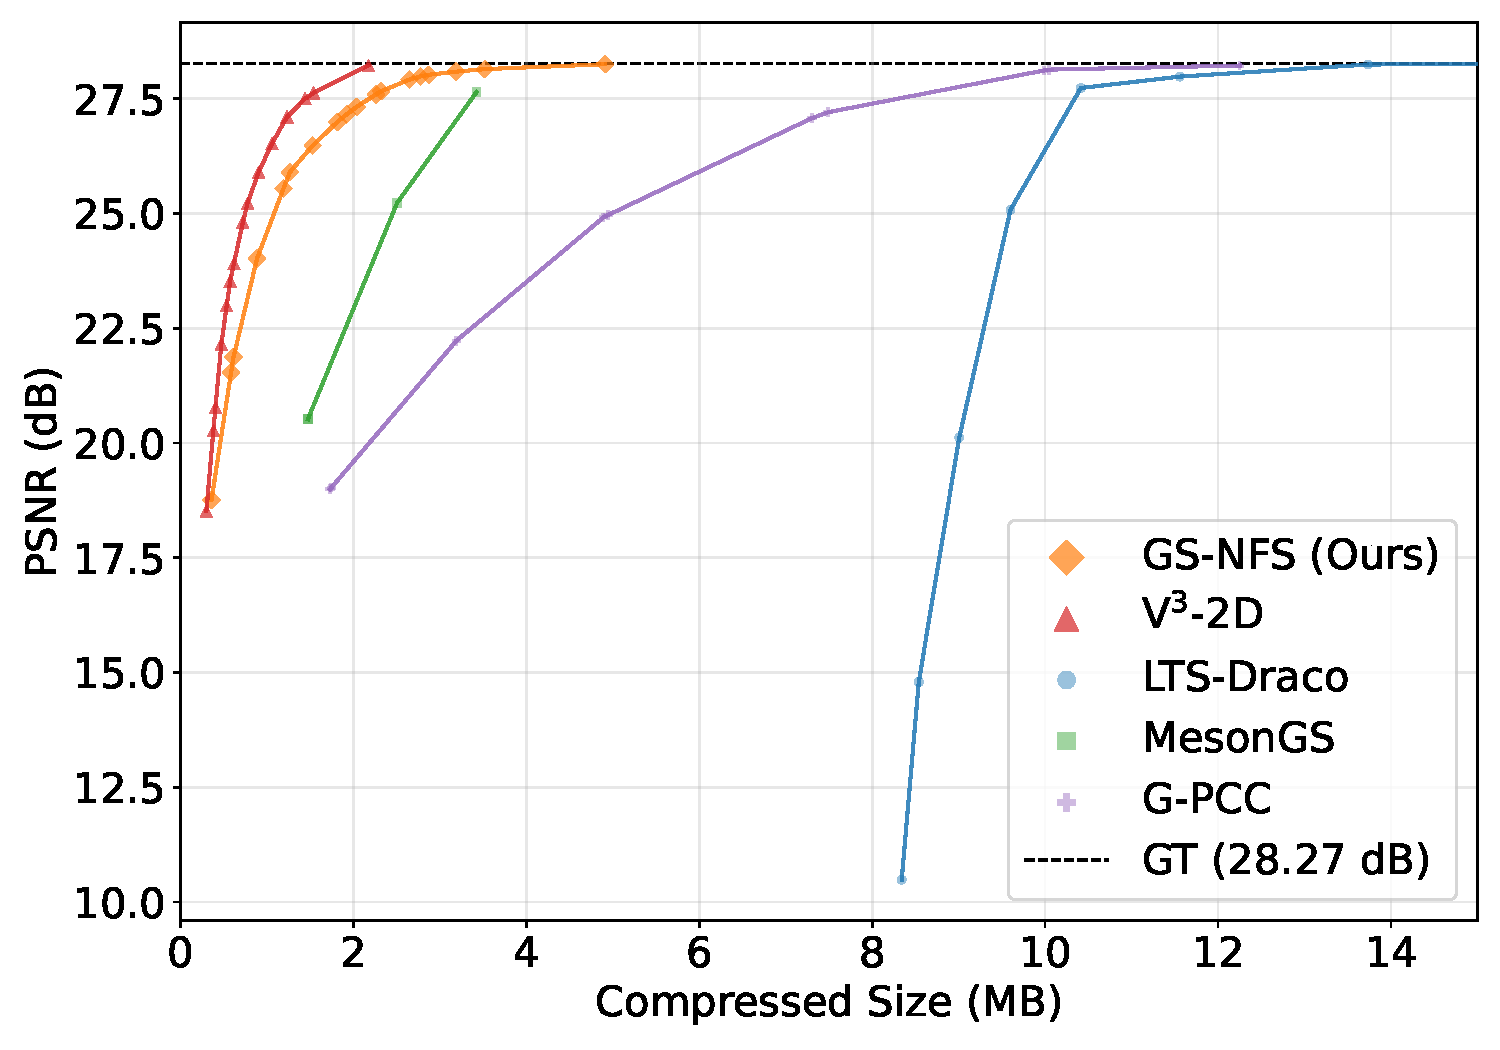
\includegraphics[width=\linewidth]{figures/rd_baselines/rd_baselines_curve_flame_salmon_1_frame1.pdf}
        \caption{flame\_salmon\_1}
        \label{fig:rd-flame-salmon}
    \end{subfigure}
    \vspace{0.5em}
    \begin{subfigure}[b]{0.48\linewidth}
        \centering
        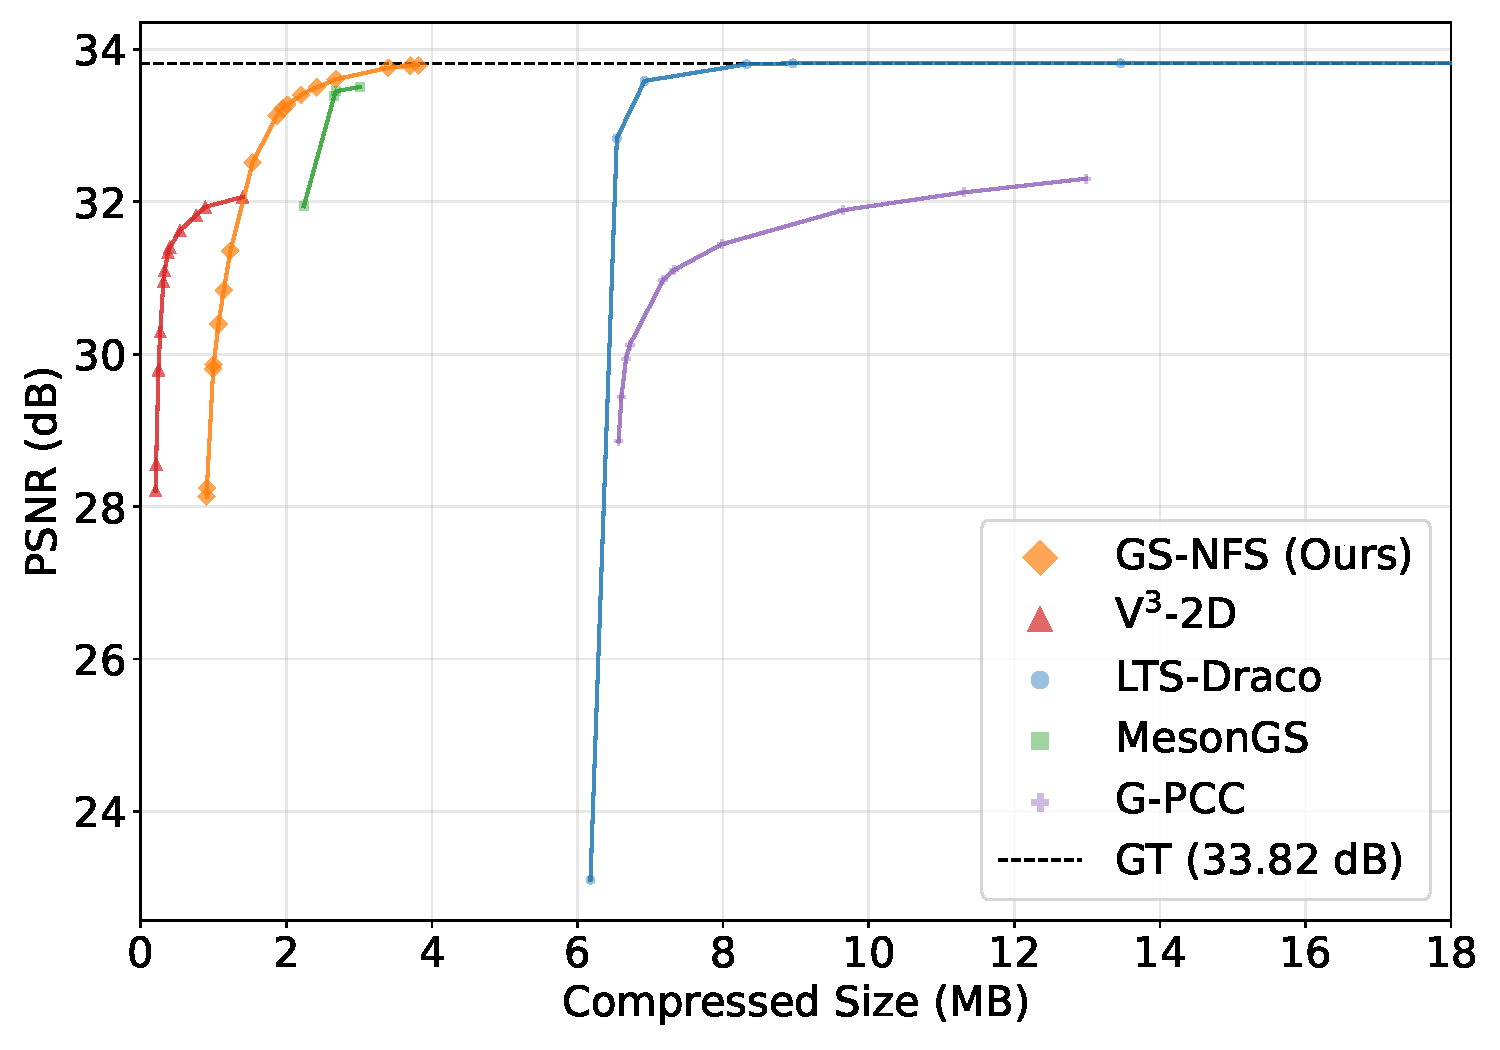
\includegraphics[width=\linewidth]{figures/rd_baselines/rd_baselines_curve_flame_steak_frame1.pdf}
        \caption{flame\_steak}
        \label{fig:rd-flame-steak}
    \end{subfigure}
    \hfill
    \begin{subfigure}[b]{0.48\linewidth}
        \centering
        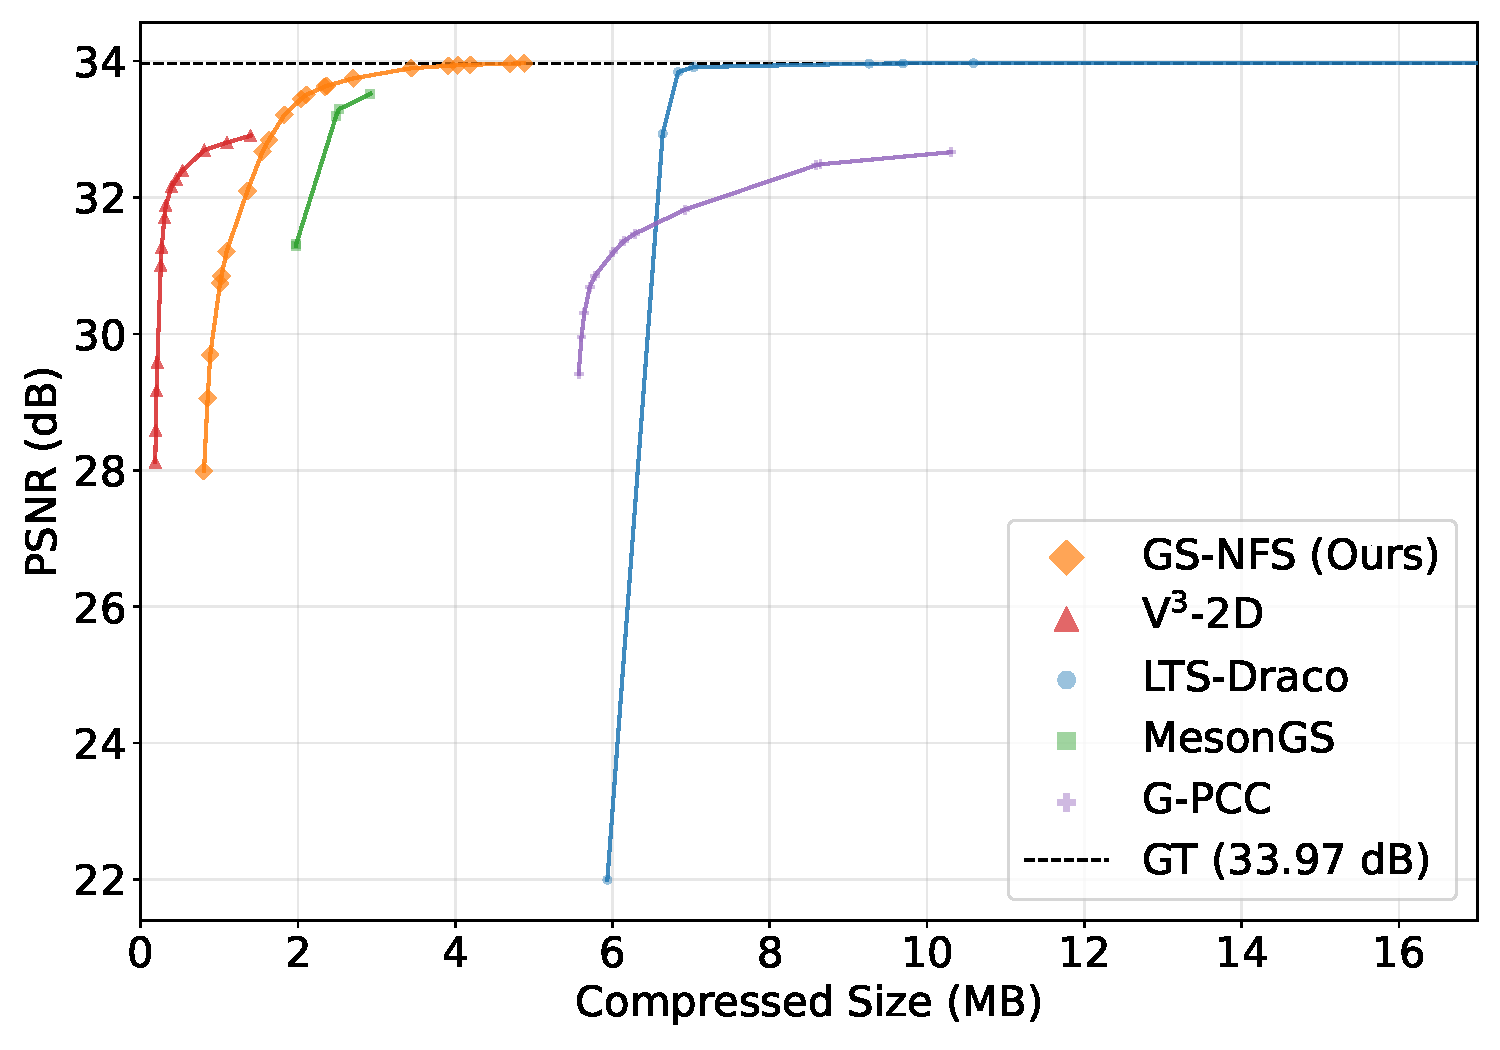
\includegraphics[width=\linewidth]{figures/rd_baselines/rd_baselines_curve_sear_steak_frame1.pdf}
        \caption{sear\_steak}
        \label{fig:rd-sear-steak}
    \end{subfigure}
    \caption{Rate-distortion curves for N3DV sequences (frame 1).}
    \label{fig:rd-baselines-n3dv}
\end{figure}

\section{Generating R-D Curves}\label{app:generating-r-d}

%\ramesh{Either put a table, or a textual description, of all the parameters we used for generating the R-D curves.}

To generate the rate-distortion (R-D) curves, we perform an exhaustive parameter sweep for each baseline codec, per frame.

For each parameter configuration, we compress and decompress the 3DGS representation of a single frame, render the decompressed Gaussians, and compute PSNR against the ground-truth renders (rendered from the uncompressed model).
%\haodong {SSIM?}

All renders use a resolution-downscale factor of ~2.

For \vthree{}-2D, which operates on groups of frames, we compress a group of 20 consecutive frames starting from the target frame and report the per-frame average compressed size; PSNR and SSIM are measured only on the target frame. 
%
All other baselines compress and evaluate a single frame independently.

The resulting (compressed size, quality) operating points are reduced to their upper convex hull to produce the final R-D curve.

Table~\ref{tab:rd-params} lists the swept parameters and their ranges for each baseline. Dataset-specific settings are noted where applicable.

\begin{table}[t]
\centering
\setlength{\tabcolsep}{3pt}
\small
\begin{tabular}{@{}llp{2.8cm}r@{}}
\toprule
\textbf{Method} & \textbf{Parameter} & \textbf{Values} & \textbf{\#} \\
\midrule
\multirow{2}{*}{V$^3$\!-2D}
  & QP         & $\{0, 1, \ldots, 40\}$           & \multirow{2}{*}{41} \\
  & Group size & 20                               & \\
\midrule
\multirow{4}{*}{MesonGS}
  & Octree depth & $\{8,10,12\}$/$\{12,14,16\}^\ast$ & \multirow{4}{*}{24} \\
  & Num.\ bits   & $\{8, 16\}$                       & \\
  & Blocks       & $\{57, 66\}$                      & \\
  & Codebook     & $\{2048, 4096\}$                  & \\
\midrule
\multirow{5}{*}{\shortstack[l]{LTS-\\Draco}}
  & \texttt{eg} (geom.)    & $\{0,8,12,16\}$        & \multirow{5}{*}{256} \\
  & \texttt{eo} (opacity)  & $\{0,8,12,16\}$        & \\
  & \texttt{et} (SH)       & $\{0,8,12,16\}$        & \\
  & \texttt{es} (scale)    & $\{0,8,12,16\}$        & \\
  & Comp.\ level           & 10                     & \\
\midrule
\multirow{2}{*}{G-PCC}
  & Octree depth & $\{8\text{--}12\}$/$\{12\text{--}17\}^\ast$ & \multirow{2}{*}{\shortstack[r]{225/\\270$^\ast$}} \\
  & $(q_r,q_d,q_o)^\dagger$ & 45 selected triples           & \\
\bottomrule
\end{tabular}
\vspace{2pt}
\raggedright
{\scriptsize $^\ast$\,HiFi4G\,/\,N3DV. G-PCC total = octree depths $\times$ 45 QP triples.\\
$^\dagger$\,$q_r$: QP for remaining attributes, $q_d$: QP for DC coefficients, $q_o$: QP for opacity.}
\caption{Parameter sweep configurations for R-D curve generation.}
\label{tab:rd-params}
\end{table}

\section{Compressing Static Scenes}\label{app:compr-stat-scen}

\begin{table}[t]
  \centering
  \footnotesize
  \scalebox{0.9}{
  \begin{tabular}{l|l|rr|rrr}
    \hline
    \textbf{Scene} & \textbf{Method} & \textbf{Enc.} & \textbf{Dec.} & \textbf{PSNR} & \textbf{Size} \\
    & & (ms) & (ms) & (dB) & (MB) \\
    \hline\hline
    \multirow{4}{*}{\textit{drjohnson}}
      & LTS-Draco            & 5,084    & 2,610   & 35.5 & 312.8 \\
%      & Compact3D            & 423,988  & 826     & 34.7 & 0.95 & 45.6 \\
      & MesonGS              & 220,066  & 22,421  & 32.6 & 40.6 \\
%      & MesonGS (w/ prune)   & 194,248  & 14,154  & 32.2 & 0.93 & 25.2 \\
      & \textbf{\gsnfs{}}  & \textbf{165} & \textbf{183} & 34.4 & 37.8 \\
    \hline
    \multirow{4}{*}{\textit{truck}}
      & LTS-Draco            & 3,385    & 1,792   & 23.1 & 204.0 \\
%      & Compact3D            & 263,896  & 403     & 23.0 & 0.89 & 30.5 \\
      & MesonGS              & 319,395  & 14,357  & 22.7 & 27.8 \\
%      & MesonGS (w/ prune)   & 307,964  & 7,179   & 22.4 & 0.87 & 17.8 \\
      & \textbf{\gsnfs{}}  & \textbf{91} & \textbf{108} & 22.4 & 19.0 \\
    \hline
  \end{tabular}
  }
  \caption{Static \gs{} scene compression. PSNR, SSIM, and LPIPS computed on rendered test views.}
  \label{tab:static-scenes}
\end{table}

\parab{Static \gs{} scene compression.}
%
We evaluate \gsnfs{} on two large static outdoor scenes from the Deep Blending dataset (\textit{drjohnson}, ~3M Gaussians, 748~MB) and Tanks \& Temples (\textit{truck}, ~2M Gaussians, 485~MB).
%
%% We compare against LTS-Draco, MesonGS (with and without pruning), and Compact3D~\cite{morgenstern2024compact3d} (which maps sorted Gaussians to PNG images using PLAS~\cite{morgenstern2024compact3d}).
%
\cref{tab:static-scenes} shows the results.
%
\gsnfs{} achieves encode times of $91$--$165$~ms, which is \textbf{$\boldsymbol{31\times}$ faster} than LTS-Draco and \textbf{$\boldsymbol{1{,}200}$--$\boldsymbol{3{,}400\times}$ faster} than MesonGS.
%
At quality comparable to LTS-Draco ($<$1~dB PSNR difference), \gsnfs{} produces compressed files that are $5$--$10\times$ smaller.
%
%% MesonGS achieves the highest compression ratio through aggressive pruning and VQ, but at severe quality ($-3$~dB PSNR) and latency penalties.
%% %
%% Compact3D achieves worse compression than \gsnfs{}, achieves comparable quality but requires minutes for the PLAS sorting and K-means clustering steps.

\section{Other Ablations}\label{app:other-ablations}

\begin{table}[t]
  \centering
  \footnotesize
  \scalebox{0.9}{
  \begin{tabular}{l|l|rr|r}
    \hline
    \textbf{Sequence} & \textbf{Method} & \textbf{Enc. (ms)} & \textbf{Dec. (ms)} & \textbf{Size (KB)} \\
    \hline\hline
    \multirow{3}{*}{longdress}
      & Draco (CPU)       & 126  & 57  & 395 \\
      & G-PCC (CPU)        & 195  & 97  & 195 \\
      & \gsnfs{} octree & \textbf{2.9}  & \textbf{1.9} & 238 \\
    \hline
    \multirow{3}{*}{soldier}
      & Draco (CPU)       & 170  & 79  & 533 \\
      & G-PCC (CPU)        & 268  & 136 & 273 \\
      & \gsnfs{} octree & \textbf{3.4}  & \textbf{2.4} & 332 \\
    \hline
    \multirow{3}{*}{band2}
      & Draco (CPU)       & 123  & 54  & 561 \\
      & G-PCC (CPU)        & 325  & 213 & 526 \\
      & \gsnfs{} octree & \textbf{3.3}  & \textbf{2.6} & 565 \\
    \hline
    \multirow{3}{*}{pizza1}
      & Draco (CPU)       & 137  & 59  & 617 \\
      & G-PCC (CPU)        & 343  & 222 & 572 \\
      & \gsnfs{} octree & \textbf{3.3}  & \textbf{2.6} & 616 \\
    \hline
  \end{tabular}
  }
  \caption{Position-only octree encoding on point-cloud sequences. Encode/decode in ms, size in KB, averaged per frame.}
  \label{tab:ptcl-octree}
\end{table}
%

\parab{GPU vs.\ CPU octree encoding.}
%
We compare \gsnfs{}'s GPU octree encoder against Draco~\cite{draco} and G-PCC~\cite{gpcc} for position-only compression.
%
%% For a fair comparison, we extract positions from \gs{} PLY files, voxelize them (timing not included), and run all three codecs.
%
\cref{tab:ablation-octree} shows that \gsnfs{}'s GPU octree encoding time is \textbf{16-34$\boldsymbol\times$ faster} ($8$--$14\times$ for decoding) than Draco and \textbf{70--100$\boldsymbol\times$ faster} than G-PCC for encoding ($50$--$65\times$ for decoding), while producing bitstreams of comparable size.
%
ANS entropy coding of the octree occupancy bytes adds only ${\sim}0.3$~ms but roughly halves the compressed size.

\parab{RLGR parallelization.}
%
\begin{table}[t]
  \centering
  \footnotesize
  \begin{tabular}{l|rr|r|r}
    \hline
    \textbf{Variant} & \textbf{Block size} & \textbf{Enc.\ (ms)} & \textbf{Dec.\ (ms)} & \textbf{$\Delta$Size} \\
    \hline\hline
    CPU &  --   & 143.8  & 207.1 & 0.0\% \\
    GPU &  --   & 494.2  & 447.4 & 0.0\% \\
    GPU & 8192  & 15.7  & 15.0   & 0.1\% \\
    GPU & 4096  & 8.0   & 7.6    & 0.2\% \\
    GPU & 2048  & 4.1   & 4.0    & 0.4\% \\
    GPU & 1024  & 2.9   & 2.4    & 0.8\% \\
    GPU & 512   & 2.5   & 1.9    & 1.5\% \\
    GPU & 256   & 2.5   & 2.1    & 2.5\% \\
    \hline
  \end{tabular}
  \caption{RLGR entropy coding latency: CPU vs.\ GPU with varying block sizes for flame\_salmon.}
  \label{tab:ablation-rlgr}
\end{table}
%
\gsnfs{} parallelizes RLGR entropy coding by partitioning each attribute channel into fixed-size blocks and encoding them independently on GPU threads (\cref{sec:quant-entr-coding}).
%
\cref{tab:ablation-rlgr} compares the CPU baseline (sequential per-channel RLGR) against GPU variants with different block sizes.
%
Parallel RLGR a block size of $512$ achieves a \textbf{$\boldsymbol{58\times}$ encode} and \textbf{$\boldsymbol{109\times}$ decode speedup} on a desktop GPU over CPU, with only ${\sim}1.5$\% increase in compressed size.
%
On Jetson Orin, a block size of $512$ achieves ${\sim}6$~ms decode time per frame, compared to ${\sim}180$~ms for the CPU implementation--a $30\times$ speedup.
%
Smaller block sizes below 512 starts having diminishing returns.
%
Block size 2048--8192 provides a balanced tradeoff: $18$--$51\times$ speedup in encode/decode latency with negligible size overhead.

\begin{table}[t]
  \centering
  \footnotesize
  \scalebox{0.9}{
  \begin{tabular}{l|l|rr|r}
    \hline
    \textbf{Sequence} & \textbf{Method} & \textbf{Enc.\ (ms)} & \textbf{Dec.\ (ms)} & \textbf{Comp Ratio} \\
    \hline\hline
    \multirow{4}{*}{\begin{tabular}[c]{@{}l@{}}flame\_salmon\\ (400K Gauss)\end{tabular}}
      & Draco (CPU)                 & 98.0          & 37.5            & 10.9$\times$ \\
      & G-PCC (CPU)                  & 228.6         & 127.5           & 11.3$\times$ \\
      & Octree (w/o ANS) & 2.9           & 2.4           & 6.6$\times$ \\
      & Octree (w/ ANS)  & \textbf{3.2}  & \textbf{2.7}  & 11.2$\times$ \\
    \hline
    \multirow{4}{*}{\begin{tabular}[c]{@{}l@{}}sear\_steak\\ (250K Gauss)\end{tabular}}
      & Draco (CPU)                 & 64.9          & 28.1          & 5.1$\times$ \\
      & G-PCC (CPU)                  & 294.8         & 204.3         & 5.2$\times$ \\
      & Octree (w/o ANS) & 2.9           & 3.0           & 2.5$\times$ \\
      & Octree (w/ ANS)  & \textbf{3.2}  & \textbf{3.1}  & 4.8$\times$ \\
    \hline
    \multirow{4}{*}{\begin{tabular}[c]{@{}l@{}}Actor1\\ (130K Gauss)\end{tabular}}
      & Draco (CPU)                     & 30.7          & 13.0          & 6.7$\times$ \\
      & G-PCC (CPU)                      & 127.8         & 91.2          & 6.8$\times$ \\
      & Octree (w/o ANS)     & 1.8           & 1.4           & 3.4$\times$ \\
      & Octree (w/ ANS)      & \textbf{1.9}  & \textbf{1.6}  & 6.1$\times$ \\
    \hline
  \end{tabular}}
  \caption{Octree compression: CPU-based methods vs \gsnfs{}'s octree codec.}
  \label{tab:ablation-octree}
\end{table}

\begin{table}[t]
  \centering
  \footnotesize
  \scalebox{0.8}{
  \begin{tabular}{l|l|r|rr|r}
    \hline
    \textbf{Sequence} & \textbf{SH degree} & \textbf{Tot. ch} & \textbf{PyTorch (ms)} & \textbf{CUDA (ms)} & \textbf{Speedup} \\
    \hline\hline
    Actor1         & 0 & 11 & 77  & 20 & 3.9$\times$ \\
    Actor1         & 3 & 56 & 100 & 28 & 3.6$\times$ \\
    flame\_salmon  & 0 & 11 & 101 & 31 & 3.3$\times$ \\
    flame\_salmon  & 2 & 35 & 125 & 57 & 2.2$\times$ \\
    sear\_steak    & 0 & 11 & 79  & 25 & 3.2$\times$ \\
    sear\_steak    & 2 & 35 & 96  & 47 & 2.0$\times$ \\
    \hline
    \end{tabular}
  }
  \caption{RAHT decode latency on Jetson Orin (ms). CUDA vs.\ PyTorch implementation. Averaged across sampled frames.}
  \label{tab:jetson-raht-decode}
\end{table}

\begin{table}[b]
  \centering
  \footnotesize
  \begin{tabular}{l|rrr|rr}
    \hline
    & \multicolumn{3}{c|}{\textbf{Compressed Size (MB)}} & \multicolumn{2}{c}{\textbf{Relative Ratio}} \\
    \textbf{Sequence} & RGB & YUV & KLT & RGB/KLT & YUV/KLT \\
    \hline\hline
    flame\_salmon  & 11.94 & 11.37  & 8.35  & 1.43  & 1.36  \\
    sear\_steak    & 9.29 & 8.99  & 6.78    & 1.37  & 1.33  \\
    Actor1         & 10.97 & 10.43  & 9.90  & 1.11  & 1.05  \\
    \hline
  \end{tabular}
  \caption{Impact of color decorrelation on compressed size (megabytes).}
  \label{tab:ablation-klt}
\end{table}